\chapter*{Notational conventions}
This section will briefly introduce the notational conventions used in this book. As is common in sign language linguistics, manual signs are glossed using small capitals (e.\,g., \textsc{sign}). All glosses are in English (irrespective of the sign language). If the English translation consists of several words, but only a single sign is used, this is indicated by hyphens. The sign \textsc{perform-magic}, for example, is a single sign, but English requires a multi-word expression. Compounds are indicated by hash signs (e.\,g., \textsc{police\#person} `police man'). Pointings used as pronouns or to localize absent referents are glossed \textsc{index}. Subscripts indicate the direction of indices in signing space: 1 $=$ towards the signer's chest, 2 $=$ towards the addressee, 3 $=$ towards some other point in signing space. To distinguish between different points in space, lower case letters are used (\textsc{index}\textsubscript{3a}, for example, could be one point in space to be differentiated from \textsc{index}\textsubscript{3b}). Possessive pronouns are glossed \textsc{poss}, again using indices (e.\,g., \textsc{poss}\textsubscript{1} means `my', \textsc{poss}\textsubscript{2} means `your'). Similar indices are used when referring to verb signs moving from one location in space to another. Thus, the gloss \textsubscript{1}\textsc{give}\textsubscript{2} is to be interpreted as the sign meaning `to give' moving from the signer’s location to the location of the addressee. 

Addition symbols are used for indicating reduplications\is{reduplication}. Thus \textsc{person}++ means that the sign for `person' is produced twice and \textsc{person}+++ means that the sign is produced three times. Other modifications of the movement path of signs are indicated using subscripts. An example would be \textsc{go}\textsubscript{durative} meaning that the sign for `to go' is modified for durative aspect. The exact form the modification takes will be described in the main text if necessary.

There are several manual signs with special names. Among them is the sign \textsc{pam} (`person agreement marker') which is usually analyzed as a type of auxiliary verb expressing agreement (in Section \ref{dom} I will argue that it is a preposition instead). An example sentence is \textsc{paul angry pam maria} `Paul is angry at Maria'. Another sign with a name of its own is \textsc{bem} which is analyzed as a benefactive\is{benefactive} marker. It can be translated as `for' in most cases. An example sentence is \textsc{paul bem maria cake bake} `Paul bakes a cake for Maria'. The last sign with its own name I want to briefly mention is \textsc{p-ug},\is{palm-up gesture} an abbreviation standing for `palm-up gesture'\is{palm-up gesture} produced one- or two handedly with the palms facing upwards. This sign, often appearing clause-finally in questions, has an unclear status between a sign and a gesture and will be discussed in Sections \ref{polargeneralsectionlabel} and \ref{constint}. 

Non-manual markers, i.\,e., markers which are not produced with the hands, but simultaneously with manual material, for example, with the face or the shoulders, are glossed using lines marking their on- and offsets. An example is given in (\ref{pugdgsnotationalconv}).\is{palm-up gesture}

%\item \label{ex34}
%\slg{ix}\textsubscript{3a} \slg{light there}\slg[hn,es]{*peter at-home must} \\
%`The light is on. Peter must be at home.'\hfill (\cite{bross}, p.194)

\begin{exe}
\ex\label{pugdgsnotationalconv}
\slg[wh]{maria angry pam who p-ug}
\glt `At whom is Maria angry?' \label{ex:pugdgsa} 
\end{exe}



%\begin{exe}
%\ex\label{pugdgsnotationalconv}
%{\hspace{148pt}wh}  \\
%{$\overline{\textrm{\textsc{maria angry pam who p-ug}}}$}
%\glt `At whom is Maria angry?' \label{ex:pugdgsa} 
%\end{exe}

\noindent The line above the manual signs indicates that the whole clause is accompanied by a non-manual marking glossed `wh'. The exact articulation of the non-manuals will be described in the main text. 

\end{document}


\begin{theo}[Iconicity and the Bodily-Mapping Hypothesis]\label{iconicity}
\is{iconicity|(}
\vspace{-0.3cm}\linebreak
\noindent Earlier I claimed that the hypothesized mapping of scope onto the body could be called iconic. As iconicity is often understood as a transparent relation between a concrete meaning and form at a morphological, lexical, or syntactic level, and not as a mapping between an abstract meaning (scope) and form (the body), I will make some brief remarks on the term as it is used here. \citet[20]{taub2004iconicity}, for example, notes that with iconic items, ``some aspect of the item's physical form (shape, sound, temporal structure, etc.) resemble a concrete sensory image''. The problem with this definition is that it is constrained to an ``item's physical form'' and thus excludes more abstract uses of the term. For this reason, I will adopt a broader definition of iconicity based on \citet{jespersen1922language} and \citet{jakobsonwaugh1979soundshape}. \citet[396]{jespersen1922language} defines iconicity (or sound symbolism)  as ``a natural correspondence between sound and sense''. Similarly, \citet[178]{jakobsonwaugh1979soundshape} define it as ``a natural similarity association between sound and meaning''. Of course, this definition, again, is too narrow as it is constrained to sound. 

If we take the organization of the clausal spine as `natural' in a way that it is (presumably) shared by all languages and if we take iconicity to be `a natural similarity association between linguistic form and meaning' the bodily-mapping hypothesis states that sign languages iconically map syntactic structures onto the body. There are two more notes to make. First, the similarity between syntax and the body lies in the fact that both are organized in a hierarchical way. Thus, structures located higher up in the clausal spine take scope over lower structures. Similarly, articulators in sign languages located higher up on the body take scope over expressions encoded by lower articulators. The second note concerns the term `meaning'. As this term is used in a fairly broad sense here, I will clearly state which kind of meanings we are concerned here: As iconicity is understood as a relationship between form and meaning, the bodily-mapping hypothesis is an hypothesis about the height or an articulator (the linguistic form) and the height (or: width) of the scope an operator takes (meaning).

Iconicity, of course, usually relates a linguistic form to an extra-linguistic meaning. In this case, however, it is a linguistic form that relates to a linguistic meaning. In this way, the iconicity of the proposed mapping principle is different from many cases of iconicity discussed in the linguistic literature.


\is{iconicity|)}

\end{theo}

\noindent There seems to be no possibility to express lexical concepts via facial articulators (only) in sign languages. Instead, manual sign must be used, although the signs for concrete actions like smiling or crying indeed have their places of articulation in the face. 

If Bross \& Hole's hypotheses are correct, this will mean that neighboring categories will find similar expression. I call the principle that neighboring categories, i.\,e., categories which are adjacent in the syntax, find similar expression in a language the `principle of analogical designation' (see the following excursus).\footnote{ For a similar observation regarding syncretism in the case hierarchy, see \citet{caha2009nanosyntax} and for compounding see \citet{hole2015arguments}.}

\begin{savenotes}
\begin{theo}[The Principle of Analogical Designation]
\is{analogical designation|(}
\vspace{-0.3cm}\linebreak
\noindent What\label{analogicaldesignation} can be derived from the observations made by \citet{bross2017scope}, if they are indeed correct, is that neighboring categories on the Cinquean hierarchy (introduced in detail in Chapter \ref{ipsystem}) are expressed in similar ways, i.\,e. by using adjacent body parts: the nearer two categories are in the hierarchy, the nearer their expression will be on the body. I call this idea that syntactic proximity is mirrored by phonological similarity the `principle of analogical designation'. We find similar ideas all over the history of linguistics. Otto Behaghel, for example, famously stated that elements which belong close together conceptually will also be placed close together in a sentence.\footnote{ \, The original quote reads ``Das oberste Gesetz ist dieses, da\ss\ das geistig eng Zusammengeh\"orige auch eng zusammengestellt wird'' \citep[4]{behaghel1932}.} While Behaghel's First Law is concerned with the placement of words and phrases in clauses, the principle of analogical designation is concerned with the expression of grammatical categories \textit{per se}. It thus resembles more Wilhelm von Humboldt's observation that related concepts are likely to be expressed phonologically similar cross-linguistically: ``Since \textit{words} always correspond to \textit{concepts}, it is natural for \textit{related concepts} to be designated by \textit{related sounds}.''\footnote{ \textcolor{white}{n}The original quote reads: ``Da \textit{W\"orter} immer \textit{Begriffen} gegen\"uberstehen, so ist es nat\"urlich, \textit{verwandte Begriffe} mit \textit{verwandten Lauten} zu bezeichnen.'' \citet[75]{von1836kawi}. Note that Humboldt also explicitly uses the word `analogy' when talking about ``designation'' and an ``analogy of concepts and sounds'' (the German original: ``Man kann diese Bezeichnung, in welcher die Analogie der Begriffe und der Laute\dots\ die \textit{analogische} nennen'' \citet[81]{von1836kawi}; the English translations were taken from \citet{humboldt1999language}. All emphases in original. } The general idea of the principle of analogical designation can be compared to the Nanosyntactic *ABA theorem stating that only adjacent categories can undergo syncretism (see, for example, \citealt{bobalji2007comparative,bobalji2012universals,caha2009nanosyntax}.)

While I will shed some light on the principle of analogical designation in the course of this book, there is much more work to do. It sometimes seems as if the expression of some categories can jump over larger portions of the tree, although not completely random: Many languages, for example, use the same modal verbs to express different kinds of modality (e.\,g., epistemic or deontic modality). Suppose we have three different kinds of modality, A, B, and C hierarchically ordered as A $>$ B $>$ C. While I would propose that it is unlikely that a language uses the modal verb x to express A and C, but another modal to express B, as this would violate the principle of analogical designation, it is unclear why the principle should hold in the first place as there are many other grammatical categories intervening between the different modalities which do not find similar expressions. 

\is{analogical designation|)}
\is{principle of analogical designation|see{analogical designation}}

\end{theo}
\end{savenotes}

\noindent While \citet{bross2017scope} have found evidence that the high-scoping speech-act operators (indicating that a clause is to be understood as a question, an imperative, etc.), the evaluation as good or bad, and epistemic modality are expressed non-manually with upper-face articulators in DGS, \is{scalarity}scalarity (the evaluation as being much or little, see Hole 2015) is produced non-manually with the lower face. Additionally, they have shown that even lower categories---those below tense---, like volition, deontic, and root modality are produced manually only. While they take volition to be expressed by employing a left-to-right-concatenation strategy, they claim that root modals concatenate from right to left---while deontic modals seem to allow both strategies and, thus, present an unclear picture (for an exact description of why some of these categories are higher and others are lower see Chapter \ref{ipsystem}).

An additional claim by \citet{bross2017scope} was that the general split between categories above and below tense is not only a split between layering and concatenation, but also a semantic split between meanings which do not directly contribute to truth conditions (not-at-issue meaning) and meanings which do contribute to truth conditions (at-issue meaning) (see \citealt{simons2010projects, tonhauser2013toward}). This claim has far reaching theoretical consequences as it is not a purely semantic claim, but a syntactic one as it states that the at-issue/not-at-issue divide is hardwired into syntax: not-at-issue meanings are the meanings expressed by the categories above tense, while at-issue meaning is the meaning contributed by the categories below tense. This hypothesis is restated in (\ref{atissuenotatissuedivide}).

\begin{exe}
\ex \textit{The at-issue/not-at-issue divide hypothesis} \\
The split between categories expressing not-at-issue and at-issue meanings is hardwired into syntax: Categories above tense are not-at-issue while categories below tense are at-issue.\label{atissuenotatissuedivide} In sign languages, this split finds visible effects as categories above tense find their expression via non-manual markings and categories below tense are marked manually.
\end{exe}

\noindent I will discuss this hypothesis in more detail in Section \ref{atnotissue} where I will review some DGS data and show that non-manual expressions indeed always contribute not-at-issue meanings. 

While \citet{bross2017scope} only looked at some clausal categories, this book is an attempt to broaden the picture by investigating the whole range of clausal categories in the CP, IP/TP, and VoiceP domain and put their claims to test (with VoiceP being the highest verbal layer introducing the agent in its specifier). For this reason this book is organized into three main chapters, one devoted to each of the three clausal layers. 

Beside the four main claims, (i) the \is{bodily-mapping hypothesis}bodily-mapping hypothesis in the narrow sense, (ii) that categories below tense are expressed by a manual left-to-right-concatenation strategy, that (iii) even lower categories are expressed by a right-to-left concatenation strategy, and (iv) the at-issue/not-at-issue divide hypothesis, I hypothesize that lower aspectual categories which modify the event itself are again expressed by layering, but by a special form of layering I call `lower layering' or `inner layering'.\is{lower layering}\is{inner layering|see{lower layering}} To be more precise, I observe that aspectual categories below VoiceP are expressed by manipulating the movement path of the verb sign (i.\,e., there is a simultaneous expression of the verb and an aspectual category):

\begin{exe}
\ex \textit{The VoiceP-internal modulation hypothesis:}\is{VoiceP-internal modulation hypothesis}\\
Aspectual categories below the VoiceP (the so-called `inner aspects')\is{inner aspect} do not find their expression by adding manual signs, but by modulating the movement path of the verb sign. \label{vpinternalmodhyp}
\end{exe}

\noindent This hypothesis will be put to test in the IP and VoiceP parts of the book (i.\,e., Chapters \ref{ipsystem} and \ref{insidevp}). Taken together, there are five guiding hypotheses which will be put to test while going through the clause structure of German Sign Language throughout the book. In summary, the proposal looks as in (\ref{treeovervies}) (see next page). The tree shows the basic structure of DGS, following the basic assumptions presented in Section \ref{basicclausstructuredgs} (all heads are final for now) extended by the higher and lower aspectual categories described in \citet{cinque1999adverbs, cinque2006restructuring}. Note that the tree only shows the highest outer and inner aspects. The complement branches of the two aspects are dotted to indicate that other aspectual categories are left out.

The tree depicts the assumption that the higher categories will be expressed by way of layering, while the higher, IP-internal aspectual categories (called `outer aspects') find manual expression and the lower aspectual categories (the `inner aspects')\is{inner aspect}, located below VoiceP find their expression by modulating the movement path of the verb sign (probably, the verb moves into the corresponding aspectual projection in the case of inner aspect). 

\begin{exe}
\ex\label{treeovervies}
\begin{minipage}[t]{\linewidth}
          \raggedright
          \adjustbox{valign=t}{%
            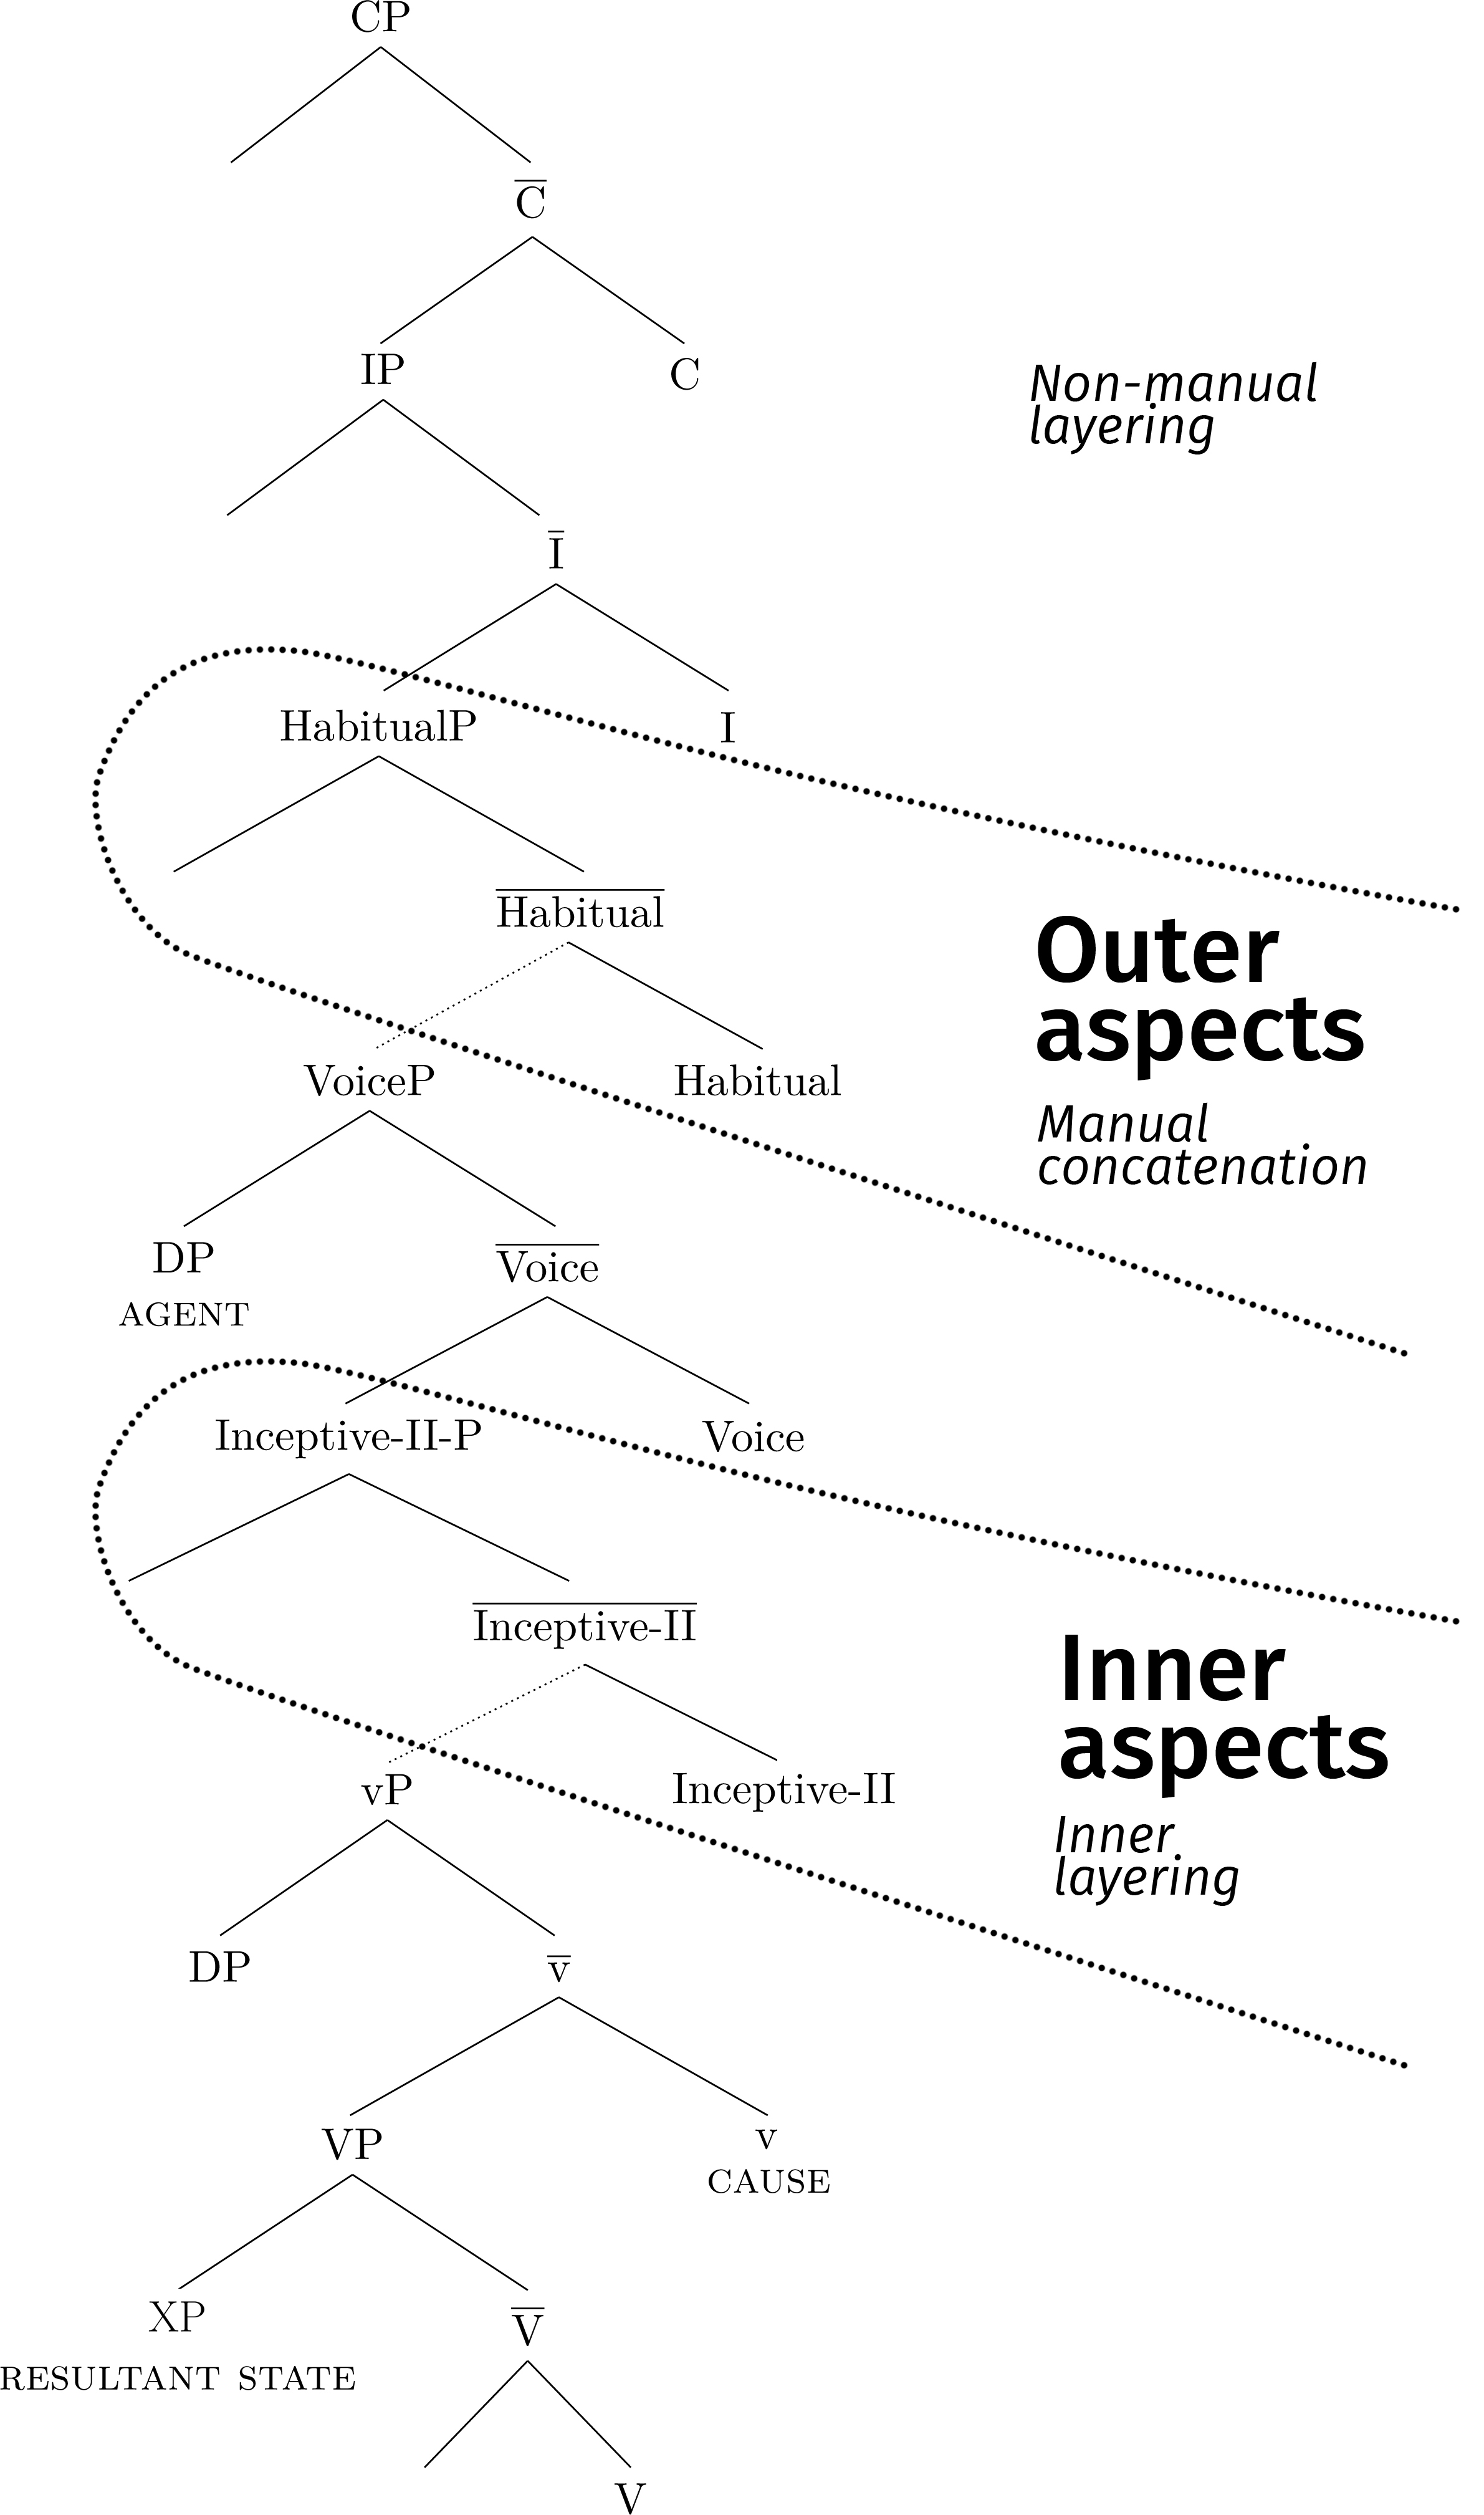
\includegraphics[width=0.88\linewidth]{tree.jpg}%
          }
    \end{minipage}
\end{exe}
